\chapterbackmatter{Solutions to Supplementary Exercises}

\begin{enumerate}
\SupplementarySolution{1}{Canonical Dimensions in Arbitrary Dimension and A \(Z_2\)-Even Scalar Operator Census}
\begin{enumerate}
\item
The action is dimensionless, so every Lagrangian density has dimension
\(D\).  The scalar and gauge kinetic terms and the Dirac kinetic term give
\[
 2+2[\phi]=D,\qquad 2+2[A]=D,\qquad
 1+2[\psi]=D.
\]
Consequently
\[
 [\phi]=[A_\mu]=\frac{D-2}{2},\qquad
 [\psi]=\frac{D-1}{2},\qquad [F_{\mu\nu}]=\frac D2.
\]
The operator in the question has
\[
 d_{\mathcal O}=r+\frac{D-2}{2}n_\phi
 +\frac{D-1}{2}n_\psi+\frac D2n_F,
 \qquad [C_{\mathcal O}]=D-d_{\mathcal O}.
\]
Under a dilation toward low energy its dimensionless coupling is multiplied
by \(b^{D-d_{\mathcal O}}\).  Thus \(d_{\mathcal O}<D\) is relevant,
\(d_{\mathcal O}=D\) is marginal, and \(d_{\mathcal O}>D\) is irrelevant at
the Gaussian fixed point.  Quantum anomalous dimensions can refine this
classification, but do not alter the canonical result.
\item
Before eliminating redundancies, convenient representatives are
\[
\begin{array}{c|l}
d&\text{operators}\\ \hline
0&1\\
2&\phi^2\\
4&(\partial\phi)^2,\ \phi^4\\
6&\phi^6,\ \phi^2(\partial\phi)^2,\quad
   \phi^3\Box\phi,\ (\Box\phi)^2 .
\end{array}
\]
Integration by parts gives
\[
 \phi^3\Box\phi=-3\phi^2(\partial\phi)^2+\partial_\mu
 (\phi^3\partial^\mu\phi).
\]
The leading equation of motion has the form
\(\Box\phi=m^2\phi+\lambda\phi^3/6\), with signs adjusted to the chosen
metric.  It converts \(\phi^3\Box\phi\) into a linear combination of
\(m^2\phi^4\) and \(\lambda\phi^6\), and converts
\((\Box\phi)^2\) similarly.  A minimal basis through dimension six is
therefore
\[
 \boxed{1,\quad\phi^2,\quad(\partial\phi)^2,\quad\phi^4,\quad\phi^6.}
\]
Keeping \(\phi^2(\partial\phi)^2\) instead of \(\phi^6\) is an equally valid
basis choice; physical amplitudes cannot depend on that choice.
\end{enumerate}

\SupplementarySolution{2}{The Jacobian of a Local Field Coordinate}
The functional derivative is diagonal in position space:
\[
 \frac{\delta\phi(x)}{\delta\chi(y)}
 =\left(1+\frac{3a}{M^2}\chi^2(x)\right)\delta^{(d)}(x-y).
\]
Hence
\[
 \ln\mathcal J
 =\operatorname{Tr}\ln\left(1+\frac{3a\chi^2}{M^2}\right)
 =\delta^{(d)}(0)\int \dd^dx\,
 \ln\left(1+\frac{3a\chi^2}{M^2}\right).
\]
Dimensional regularization sets
\(\delta^{(d)}(0)=\int \dd^dk/(2\pi)^d=0\), so \(\mathcal J=1\).
With a hard cutoff, \(\delta^{(d)}(0)\sim\Lambda^d\); expanding the
logarithm produces only local terms \(\chi^{2n}\), which are absorbed into
the Wilson coefficients already allowed in the action.

The source term becomes
\[
 \int \dd^dx\,J\phi
 =\int \dd^dx\left(J\chi+\frac{a}{M^2}J\chi^3\right).
\]
Thus derivatives with respect to \(J\) insert a composite nonlinear
operator, and off-shell correlators of the named field do change.  The
path integral itself is merely rewritten, however.  Transforming the
action, source, and local Jacobian consistently leaves pole locations and
LSZ-amputated amplitudes invariant.  This is the equivalence theorem; it
does not assert equality of arbitrary off-shell Green functions.

\SupplementarySolution{3}{Tree-Level Matching of a Heavy Scalar and Matching Is Not Merely Dropping the Heavy Field}
\begin{enumerate}
\item
Put \(K=M^2-\Box\).  Completing the square gives
\[
 \frac12H K H+\frac{\kappa}{2}H\phi^2
 =\frac12\left(H+\frac{\kappa}{2}K^{-1}\phi^2\right)
 K\left(H+\frac{\kappa}{2}K^{-1}\phi^2\right)
 -\frac{\kappa^2}{8}\phi^2K^{-1}\phi^2.
\]
Thus \(H_{\rm cl}=-(\kappa/2)K^{-1}\phi^2\) and
\[
 \Delta\mathcal L_{\rm eff}
 =-\frac{\kappa^2}{8}\phi^2\frac1{M^2-\Box}\phi^2
 =-\frac{\kappa^2}{8M^2}\phi^4
 -\frac{\kappa^2}{8M^4}\phi^2\Box\phi^2+O(M^{-6}).
\]
After integration by parts, the second operator is
\(+\kappa^2[\partial_\mu(\phi^2)]^2/(8M^4)\).
The full four-point amplitude is the sum of heavy exchange in the three
channels.  Expanding each Euclidean denominator,
\[
 \frac1{M^2+p^2}=\frac1{M^2}-\frac{p^2}{M^4}+\cdots,
\]
reproduces precisely the contact vertex and its derivative correction.
\item
At low momentum a single heavy propagator contributes schematically
\[
 \mathcal A_{\rm full}
 =\frac{\kappa^2}{M^2+p^2}
 =\frac{\kappa^2}{M^2}
 \left(1-\frac{p^2}{M^2}+\frac{p^4}{M^4}-\cdots\right),
\]
with a sum over channels understood.  Setting \(H=0\) and adding nothing
misses the leading amplitude, so its relative error is \(O(1)\).
The induced \(\phi^4\) operator reproduces the first term and has relative
error \(O(E^2/M^2)\).  Including the dimension-six derivative correction
leaves relative error \(O(E^4/M^4)\).

The expansion is a Taylor series about zero momentum.  It fails when a
channel invariant approaches the nearest heavy pole or threshold,
\(|p^2|\sim M^2\).  Adding more local terms cannot extend the radius of
convergence through that physical singularity; the heavy degree of freedom
must then be restored.
\end{enumerate}

\SupplementarySolution{4}{Chiral Spurions and Dipole Suppression}
The dipole contains opposite chiralities:
\[
 \bar\psi\sigma^{\mu\nu}\psi
 =\bar\psi_L\sigma^{\mu\nu}\psi_R
 +\bar\psi_R\sigma^{\mu\nu}\psi_L.
\]
Under \(U(1)_L\times U(1)_R\), the first term has phase
\(e^{\ii(\alpha_R-\alpha_L)}\).  The mass spurion in
\(m\bar\psi_L\psi_R+\mathrm{H.c.}\) has the compensating transformation.
If it is the only source of chiral breaking, the Wilson coefficient must
therefore be proportional to \(m\):
\[
 \frac{c}{M}\longrightarrow \frac{c\,m}{M^2}.
\]
A generic dimension-five dipole gives a dimensionless anomalous moment of
order \(c\,m/M\), whereas the chirally protected estimate is
\[
 \delta a=O\left(c\,\frac{m^2}{M^2}\right),\qquad
 \delta\mu=O\left(\frac{e\,c\,m}{M^2}\right).
\]
Setting \(m=0\) restores the symmetry and forces the correction to vanish,
which makes the small coefficient technically natural.

\SupplementarySolution{5}{Massless \(\phi^4\) Theory at a Symmetric Subtraction Point}
\begin{enumerate}
\item
A convenient counterterm organization in the volume's convention is
\[
 \mathcal L=-\frac12(1+\delta Z)\partial_\mu\phi\partial^\mu\phi
 -\frac12\delta m^2\phi^2
 -\frac{\lambda+\delta\lambda}{4!}\phi^4.
\]
The scalar propagator, ordinary quartic vertex, two-point counterterm, and
four-point counterterm are respectively
\[
 \frac{-\ii}{p^2-\ii0},\qquad -\ii\lambda,\qquad
 -\ii(\delta Zp^2+\delta m^2),\qquad -\ii\delta\lambda.
\]
Through order \(\lambda^2\), the 1PI four-point diagrams are the tree
vertex, the one-loop bubble in each of the \(s,t,u\) channels (each with
symmetry factor \(1/2\)), and the four-point counterterm:
\begin{center}
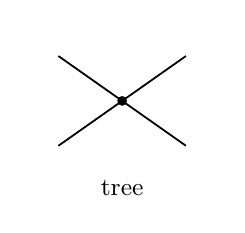
\begin{tikzpicture}[x=0.60cm,y=0.60cm,baseline=-0.5ex,line width=0.65pt,
  vertex/.style={circle,fill,inner sep=1.25pt},
  every node/.style={font=\small}]
 \path (-2.0,-2.15) (2.0,1.55);
 \coordinate (v) at (0,0);
 \draw (-1.35,0.95)--(v)--(1.35,0.95);
 \draw (-1.35,-0.95)--(v)--(1.35,-0.95);
 \node[vertex] at (v) {};
 \node at (0,-1.85) {tree};
\end{tikzpicture}
\quad
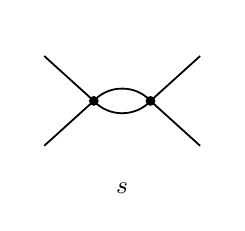
\begin{tikzpicture}[x=0.60cm,y=0.60cm,baseline=-0.5ex,line width=0.65pt,
  vertex/.style={circle,fill,inner sep=1.25pt},
  every node/.style={font=\small}]
 \path (-2.0,-2.15) (2.0,1.55);
 \coordinate (a) at (-0.60,0); \coordinate (b) at (0.60,0);
 \draw (-1.65,0.95)--(a)--(-1.65,-0.95);
 \draw (1.65,0.95)--(b)--(1.65,-0.95);
 \draw (a) to[bend left=48] (b);
 \draw (a) to[bend right=48] (b);
 \node[vertex] at (a) {}; \node[vertex] at (b) {};
 \node at (0,-1.85) {\(s\)};
\end{tikzpicture}
\quad
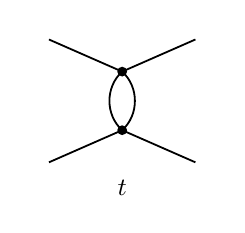
\begin{tikzpicture}[x=0.60cm,y=0.60cm,baseline=-0.5ex,line width=0.65pt,
  vertex/.style={circle,fill,inner sep=1.25pt},
  every node/.style={font=\small}]
 \path (-2.0,-2.15) (2.0,1.55);
 \coordinate (a) at (0,0.62); \coordinate (b) at (0,-0.62);
 \draw (-1.55,1.30)--(a)--(1.55,1.30);
 \draw (-1.55,-1.30)--(b)--(1.55,-1.30);
 \draw (a) to[bend left=48] (b);
 \draw (a) to[bend right=48] (b);
 \node[vertex] at (a) {}; \node[vertex] at (b) {};
 \node at (0,-1.85) {\(t\)};
\end{tikzpicture}
\quad
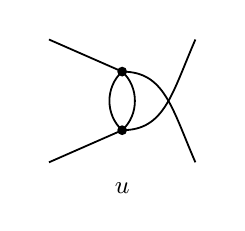
\begin{tikzpicture}[x=0.60cm,y=0.60cm,baseline=-0.5ex,line width=0.65pt,
  vertex/.style={circle,fill,inner sep=1.25pt},
  every node/.style={font=\small}]
 \path (-2.0,-2.15) (2.0,1.55);
 \coordinate (a) at (0,0.62); \coordinate (b) at (0,-0.62);
 \draw (-1.55,1.30)--(a);
 \draw (-1.55,-1.30)--(b);
 % The outgoing legs have to cross for the u channel.  Straight legs put that
 % crossing about 1.4mm from the loop, where it reads as a blot; leaving each
 % vertex horizontally first moves it three times further out.
 \draw (a) .. controls (0.90,0.62) and (1.05,-0.15) .. (1.55,-1.30);
 \draw (b) .. controls (0.90,-0.62) and (1.05,0.15) .. (1.55,1.30);
 \draw (a) to[bend left=48] (b);
 \draw (a) to[bend right=48] (b);
 \node[vertex] at (a) {}; \node[vertex] at (b) {};
 \node at (0,-1.85) {\(u\)};
\end{tikzpicture}
\quad
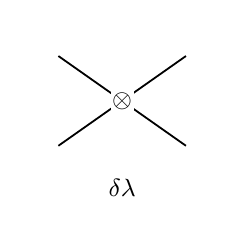
\begin{tikzpicture}[x=0.60cm,y=0.60cm,baseline=-0.5ex,line width=0.65pt,
  vertex/.style={circle,fill,inner sep=1.25pt},
  every node/.style={font=\small}]
 \path (-2.0,-2.15) (2.0,1.55);
 \coordinate (v) at (0,0);
 \draw (-1.35,0.95)--(v)--(1.35,0.95);
 \draw (-1.35,-0.95)--(v)--(1.35,-0.95);
 \node[fill=white,inner sep=0.6pt] at (v) {\(\otimes\)};
 \node at (0,-1.85) {\(\delta\lambda\)};
\end{tikzpicture}
\end{center}
  The massless
tadpole is scaleless in dimensional regularization, and the one-loop
two-point function has no momentum-dependent pole, so
\(\delta m^2=0\) and \(\delta Z=0\) at the order used here.

\item
After Wick rotation, Feynman parametrization, and a shift of loop momentum,
the bubble at a Euclidean momentum \(Q\) is
\[
\begin{aligned}
 B(Q^2)
 &\equiv \mu^\epsilon\int\frac{d^{4-\epsilon}\ell_E}
 {(2\pi)^{4-\epsilon}}
 \frac1{\ell_E^2(\ell_E+Q)^2}\\
 &=\frac1{16\pi^2}\int_0^1\dd x\left[
 \frac2\epsilon-\gamma+\ln(4\pi)
 +\ln\frac{\mu^2}{x(1-x)Q^2}\right]+O(\epsilon).
\end{aligned}
\]
Thus
\[
 \Gamma_4=-\ii\lambda
 +\frac{\ii\lambda^2}{2}\bigl[B(-s)+B(-t)+B(-u)\bigr]
 -\ii\delta\lambda+O(\lambda^3),
\]
where the arguments indicate the positive Euclidean invariants reached by
continuation.  At \(s=t=u=-M^2\),
\[
\begin{aligned}
 -\ii\lambda_{\mathrm{eff}}
 ={}&-\ii\lambda
 +\frac{\ii\lambda^2}{32\pi^2}\int_0^1\dd x\left[
 \frac6\epsilon-3\gamma+3\ln(4\pi)
 +3\ln\frac{\mu^2}{x(1-x)M^2}\right]\\
 &{}-\ii\delta\lambda+O(\lambda^3),
\end{aligned}
\]
which is the displayed form in the question after using
\(-\ii(-\ii\lambda)^2=+\ii\lambda^2\).

Choose \(\mu=M\).  Since
\(\int_0^1\dd x\,[-\ln(x(1-x))]=2\), a momentum-subtraction counterterm that
enforces \(\lambda_{\mathrm{eff}}(M)=\lambda\) is
\[
 \boxed{\;
 \delta\lambda_{\mathrm{MOM}}
 =\frac{3\lambda^2}{32\pi^2}
 \left(\frac2\epsilon-\gamma+\ln(4\pi)+2\right).
 \;}
\]
The \(\overline{\mathrm{MS}}\) choice instead removes only
\[
 \delta\lambda_{\overline{\mathrm{MS}}}
 =\frac{3\lambda^2}{16\pi^2}\frac1{\bar\epsilon},
 \qquad
 \frac1{\bar\epsilon}
 =\frac1\epsilon-\frac\gamma2+\frac12\ln(4\pi),
\]
and therefore differs by a finite redefinition of the coupling.

\item
For the renormalized 1PI \(n\)-point function the Callan--Symanzik equation
is
\[
 \left[\mu\frac{\partial}{\partial\mu}
 +\beta(\lambda)\frac{\partial}{\partial\lambda}
 +n\gamma_\phi(\lambda)\right]\Gamma^{(n)}=0.
\]
Here \(\gamma_\phi=O(\lambda^2)\), so it does not enter the one-loop
four-point calculation.  The pole part may be encoded as
\[
 \lambda_0=\mu^\epsilon\left[
 \lambda+\frac{3\lambda^2}{16\pi^2\epsilon}
 +O(\lambda^3)\right].
\]
The bare coupling is independent of \(\mu\); differentiating gives
\[
 \beta(\lambda)=-\epsilon\lambda
 +\frac{3\lambda^2}{16\pi^2}+O(\lambda^3).
\]
Taking \(\epsilon\to0\) therefore yields
\[
 \boxed{\beta(\lambda)=\frac{3\lambda^2}{16\pi^2}
 +O(\lambda^3).}
\]
\end{enumerate}

\SupplementarySolution{6}{Wilsonian Shell Integration in \(\Phi^3\) Theory}
\begin{enumerate}
\item
Use the Fourier convention
\[
 \Phi(x)=\int_{p^2<\Lambda^2}\frac{\dd^dp}{(2\pi)^d}
 e^{\ii p\cdot x}\widetilde\Phi(p).
\]
The two characteristic functions in the definition of
\(\widetilde\phi\) and \(\widetilde\chi\) partition the cutoff ball (up to
its measure-zero boundary), so
\[
 \widetilde\Phi(p)=\widetilde\phi(p)+\widetilde\chi(p).
\]
Fourier inversion immediately gives
\(\Phi(x)=\phi(x)+\chi(x)\).  Their momentum supports are disjoint, which
also makes the kinetic cross term vanish:
\(\int \dd^dx\,\partial\phi\cdot\partial\chi=0\).

\item
Expanding the cubic action gives
\[
 S[\phi+\chi]=S[\phi]+S_{\chi,0}+S_{\mathrm{int}}[\phi,\chi],
\]
where
\[
 S_{\chi,0}=\frac12\int \dd^dx\,\partial_\mu\chi\partial^\mu\chi
\]
and
\[
 \boxed{\;
 S_{\mathrm{int}}[\phi,\chi]
 =g\int \dd^dx\left(
 \frac12\phi^2\chi+\frac12\phi\chi^2+\frac1{3!}\chi^3
 \right).\;}
\]
To reproduce the functional-derivative sign printed in the question,
define
\[
 Z_\chi[J]=\mathcal N\int\mathcal D\chi\,
 \exp\left[-S_{\chi,0}-\int \dd^dx\,J\chi\right],
 \qquad Z_\chi[0]=1.
\]
Then each insertion of \(\chi(x)\) is generated by
\(-\delta/\delta J(x)\), and direct expansion of the exponential proves
\[
 e^{-W[\phi]}=e^{-S[\phi]}
 \left[
 \exp\left(-S_{\mathrm{int}}
 \left[\phi,-\frac{\delta}{\delta J}\right]\right)Z_\chi[J]
 \right]_{J=0}.
\]
Perturbation theory is obtained either by expanding this operator in powers
of \(g\) and performing Gaussian derivatives, or equivalently by using the
connected-cumulant expansion
\[
 W[\phi]=S[\phi]+\langle S_{\mathrm{int}}\rangle_>
 -\frac12\langle S_{\mathrm{int}}^2\rangle_{>,c}
 +\frac1{3!}\langle S_{\mathrm{int}}^3\rangle_{>,c}+\cdots,
\]
where every internal propagator is restricted to
\(b\Lambda<|p|<\Lambda\).

\item
Neglecting wavefunction rescaling, the diagrams relevant to the local
three-low-field vertex through order \(g^3\) are the original tree-level
cubic vertex and the one-loop triangle made from three
\(g\phi\chi^2/2\) vertices.  A vertex containing only one high-mode line
cannot contribute at zero external momentum: momentum conservation would
force that line outside the high shell.  Disconnected vacuum factors cancel
from \(W=-\ln Z\).

The connected Wick contraction is
\[
 \langle\chi^2(x)\chi^2(y)\chi^2(z)\rangle_{>,c}
 =8G_>(x-y)G_>(y-z)G_>(z-x).
\]
Its coefficient in the third cumulant is
\[
 \frac1{3!}\left(\frac g2\right)^3 8=\frac{g^3}{3!}.
\]
For external momenta small compared with the shell momenta, the triangle is
local, and hence
\[
 \frac{g_{\mathrm{eff}}}{3!}
 =\frac g{3!}+\frac{g^3}{3!}I_d+O(g^5),
 \qquad
 I_d=\int_{b\Lambda<|k|<\Lambda}
 \frac{\dd^dk}{(2\pi)^d}\frac1{(k^2)^3}.
\]
For \(\dd\neq6\),
\[
 I_d=\frac{\Omega_{d-1}}{(2\pi)^d}
 \frac{\Lambda^{d-6}-(b\Lambda)^{d-6}}{d-6}.
\]
At \(d=6\), \(\Omega_5=\pi^3\), so
\[
 I_6=\frac{\pi^3}{(2\pi)^6}\ln\frac1b
 =\frac1{64\pi^3}\ln\frac1b.
\]
Therefore
\[
 \boxed{\;
 g_{\mathrm{eff}}
 =g+\frac{g^3}{64\pi^3}\ln\frac1b+O(g^5)
 =g-\frac{g^3}{64\pi^3}\ln b+O(g^5),
 \qquad C=-\frac1{64\pi^3}.\;}
\]
\end{enumerate}

\SupplementarySolution{7}{The One-Loop Yukawa Beta Function}
Work in \(d=4-\epsilon\) and introduce
\[
 \phi_0=Z_\phi^{1/2}\phi,
 \qquad \psi_0=Z_\psi^{1/2}\psi,
 \qquad
 g_0=\mu^{\epsilon/2}Z_g g.
\]
It is useful to write the renormalized interaction and its vertex
counterterm as
\[
 \mathcal L_{\mathrm{Yuk}}
 =-\ii\mu^{\epsilon/2}gZ_1\phi\bar\psi\psi,
 \qquad Z_1=Z_gZ_\psi Z_\phi^{1/2}.
\]
With Harlow's phases, also used in the prompt, the tree-level Yukawa vertex
is \(+g\).

There are three ultraviolet computations: the fermion self-energy with one
internal fermion and one scalar, the scalar self-energy from a closed
fermion loop, and the proper Yukawa vertex triangle.  At nonexceptional
momenta their poles can all be extracted from
\[
 \mu^\epsilon\int\frac{d^{4-\epsilon}\ell_E}{(2\pi)^{4-\epsilon}}
 \frac1{(\ell_E^2+\Delta)^2}
 =\frac1{16\pi^2}\left(\frac2\epsilon+O(1)\right).
\]
For the fermion self-energy, Feynman parametrization leaves the pole
proportional to
\[
 2\int_0^1\dd x\,(1-x)\ii\slashed p=\ii\slashed p.
\]
For the scalar self-energy, the fermion trace and the two terms obtained
after the momentum shift give four times the corresponding pole in the
coefficient of \(p^2\).  The required minimal-subtraction field factors are
therefore
\[
 \boxed{\;
 Z_\psi=1-\frac{g^2}{16\pi^2\epsilon}+O(g^4),
 \qquad
 Z_\phi=1-\frac{4g^2}{16\pi^2\epsilon}+O(g^4).\;}
\]
These values give
\(\gamma_\psi=g^2/(32\pi^2)\) and
\(\gamma_\phi=g^2/(8\pi^2)\), a useful normalization check.

The divergent part of the one-loop proper vertex, relative to the
tree-level rule, is
\[
 \Gamma^{(3)}_{\mathrm{loop}}\big|_{\mathrm{UV}}
 =-g\frac{2g^2}{16\pi^2\epsilon}.
\]
It is canceled by
\[
 Z_1=1+\frac{2g^2}{16\pi^2\epsilon}+O(g^4).
\]
Consequently the coupling renormalization includes both the proper vertex
and the three external-field square roots:
\[
\begin{aligned}
 Z_g&=Z_1Z_\psi^{-1}Z_\phi^{-1/2}\\
 &=1+\frac{5g^2}{16\pi^2\epsilon}+O(g^4),
\end{aligned}
\]
and hence
\[
 g_0=\mu^{\epsilon/2}g\left[
 1+\frac{5g^2}{16\pi^2\epsilon}+O(g^4)\right].
\]
Holding \(g_0\) fixed while differentiating with respect to \(\mu\) gives
\[
 \beta_g=-\frac\epsilon2g+\frac{5g^3}{16\pi^2}+O(g^5).
\]
Thus in four dimensions
\[
 \boxed{\beta_g=\frac{5g^3}{16\pi^2}+O(g^5).}
\]

The Lagrangian displayed in the source is not, by itself, the most general
renormalizable scalar--fermion theory.  Unless an additional exact symmetry
is imposed, fermion loops require scalar-potential counterterms, including
the allowed linear, cubic, and quartic terms.  Their couplings do not enter
the one-loop pole of the Yukawa vertex or the one-loop wavefunction factors
above, so they do not change this one-loop beta function.  They must still
be included when renormalizing the full theory beyond the restricted
question.

\SupplementarySolution{8}{Euler--Heisenberg, Rayleigh Scattering, and Fermi Theory}
\begin{enumerate}
\item
Gauge invariance requires photons to occur through \(F_{\mu\nu}\).
There is no nonzero Abelian scalar cubic in \(F\), so the first
self-interactions contain four field strengths:
\[
 \mathcal O_1=(F_{\mu\nu}F^{\mu\nu})^2,\qquad
 \mathcal O_2=(F_{\mu\nu}\widetilde F^{\mu\nu})^2.
\]
Both have dimension eight.  Integrating out an electron gives
\[
 \Delta\mathcal L
 =\frac{\alpha^2}{m_e^4}(c_1\mathcal O_1+c_2\mathcal O_2)+\cdots,
\]
where \(c_i\) are numerical one-loop constants.  Each external field
strength supplies one power of photon energy, so
\[
 \mathcal A_{\gamma\gamma\to\gamma\gamma}
 =O\left(\alpha^2\frac{\omega^4}{m_e^4}\right).
\]
Two-body phase space contributes \(1/\omega^2\), yielding
\[
 \boxed{\sigma=O\left(\alpha^4\frac{\omega^6}{m_e^8}\right).}
\]
The energy power is fixed without evaluating the electron loop.
\item
For a slowly moving neutral spinless atom, the leading local interactions
are its electric and magnetic polarizabilities,
\[
 \Delta\mathcal L=h^\dagger h
 \left(c_Ea_0^3\mathbf E^2+c_Ba_0^3\mathbf B^2\right).
\]
The coefficient has dimension \(-3\), and the atomic size supplies that
scale.  Each field in a radiation wave is proportional to \(\omega\), so
\[
 \mathcal A=O(a_0^3\omega^2).
\]
The nonrelativistic scattering normalization then gives
\[
 \boxed{\sigma=O(a_0^6\omega^4).}
\]
A frequency-independent coupling would require a term linear in the
potential or a net electric charge.  Neutrality removes the charge
monopole, while gauge invariance forbids a local interaction built directly
from \(A_\mu\).  This is why the first response is a polarizability and why
shorter-wavelength light is scattered more strongly.
\item
For conserved currents the longitudinal propagator does not contribute.
The relevant factor expands as
\[
 \frac{g^2}{M^2-q^2}
 =\frac{g^2}{M^2}
 \left(1+\frac{q^2}{M^2}+O(q^4/M^4)\right),
\]
with signs changed in the Euclidean continuation.  Matching gives
\[
 \Delta\mathcal L_{\rm eff}
 =-\frac{g^2}{2M^2}J_\mu J^\mu
 -\frac{g^2}{2M^4}J_\mu\Box J^\mu+\cdots.
\]
The current has dimension three, so these are dimension-six and
dimension-eight operators.  Their matrix elements differ by
\(O(p^2/M^2)\).

The coefficient \(g^2/M^2\) may be conventionally written as a different
scale, such as \(G_F\sim1/v^2\).  The derivative series nevertheless knows
about the propagator singularity and loses convergence at \(p^2\sim M^2\),
not necessarily at \(p^2\sim v^2\).
\end{enumerate}

\SupplementarySolution{9}{Loop Power Counting and Expansion by Regions}
\begin{enumerate}
\item
Write each interaction as
\[
 \frac{c_i}{M^{d_i-4}}\mathcal O_{d_i}.
\]
A graph with \(V_i\) insertions contains the fixed factor
\[
 M^{-P},\qquad P=\sum_iV_i(d_i-4).
\]
After the heavy fields have been removed, loop denominators contain only
light masses and external momenta.  Dimensional regularization introduces
the bookkeeping scale \(\mu\), but no physical positive power of \(M\).
Consequently a loop cannot lower \(P\).  Its ultraviolet pole is a
polynomial in light momenta and masses multiplying the same \(M^{-P}\);
that polynomial is canceled by an operator at the corresponding EFT order.

For fixed \(P\), there are only finitely many nonnegative multiplicities
\(V_i\) and finitely many local operators of bounded dimension, once field
content and symmetries are fixed.  This establishes order-by-order
counterterm closure even though the complete effective Lagrangian contains
infinitely many terms.
\item
Partial fractions reduce the integral to tadpoles:
\[
 I=\frac{A(m^2)-A(M^2)}{M^2-m^2},\qquad
 A_R(a)=\frac{a}{16\pi^2}\left(\ln\frac a{\mu^2}-1\right)
\]
in the stated \(\overline{\mathrm{MS}}\) convention.  Therefore
\[
 I_R=\frac1{16\pi^2}
 \frac{m^2(\ln(m^2/\mu^2)-1)
 -M^2(\ln(M^2/\mu^2)-1)}{M^2-m^2}.
\]
With \(r=m^2/M^2\),
\[
 I_R=\frac1{16\pi^2}\left[
 1-\ln\frac{M^2}{\mu^2}
 +r\ln\frac{m^2}{M^2}+O(r^2\ln r)\right].
\]
Expanding the heavy propagator gives
\[
 \frac1{k^2+M^2}=\frac1{M^2}
 \sum_{n\geq0}\left(-\frac{k^2}{M^2}\right)^n .
\]
The resulting light tadpoles generate every \(r^n\ln m^2\) term.  They
cannot generate the analytic constants and \(\ln M^2\) pieces; those are
the Wilson coefficients obtained by matching the hard region.
\item
For
\[
 I_\alpha=\mu^{2\varepsilon}\int \dd^dk\,(k^2)^{-\alpha},
\]
the change \(k\mapsto\lambda k\) gives
\(I_\alpha=\lambda^{d-2\alpha}I_\alpha\).  With no scale that could
compensate this factor, analytic continuation sets \(I_\alpha=0\).  In the
logarithmic case the same statement may be displayed as
\[
 \int\frac{\dd^dk}{(k^2)^2}
 \propto\frac1{\varepsilon_{\rm UV}}
 -\frac1{\varepsilon_{\rm IR}}=0.
\]
The equality does not say that ultraviolet and infrared behavior are
separately absent; it says they cancel in the scaleless regulated integral.

In matching, the full theory and EFT have identical soft behavior.  If
external momenta and light masses are set to zero, common soft graphs often
become scaleless and vanish.  The remaining full-theory hard part is then
the Wilson coefficient.  Keeping track of the UV versus IR interpretation
of poles ensures that the EFT counterterm receives the correct ultraviolet
information.
\end{enumerate}

\SupplementarySolution{10}{Heavy-Vector Matching and Infrared Cancellation}
\begin{enumerate}
\item
At leading order in derivatives, write
\[
 \mathcal L_X=\frac12M^2X_\mu X^\mu
 +g_XX_\mu(J_1^\mu+J_2^\mu).
\]
The field equation gives
\[
 X_\mu=-\frac{g_X}{M^2}(J_{1\mu}+J_{2\mu})+O(M^{-4}),
\]
and substitution yields
\[
 \boxed{\;
 \Delta\mathcal L_{\rm eff}
 =-\frac{g_X^2}{2M^2}J_1^2
 -\frac{g_X^2}{M^2}J_1\cdot J_2
 -\frac{g_X^2}{2M^2}J_2^2+O(M^{-4}).\;}
\]
The cross coefficient is twice either diagonal coefficient because it
comes from expanding \((J_1+J_2)^2\).  Expanding the full exchange kernel
\(g_X^2/(q^2-M^2)\) at small \(q^2\) fixes the same relative sign.  An
overall sign changes if the quadratic-term convention changes, but the
exchange amplitude and matched contact term always agree.
\item
Single heavy exchange naturally gives
\[
 C_6^{\rm tree}\sim\frac{g_1g_2}{M^2},\qquad
 C_8^{\rm tree}\sim\frac{g_T^2}{M^4}.
\]
If symmetry or topology forbids tree generation, a one-loop coefficient is
instead
\[
 C_6^{\rm loop}\sim
 \frac{g_L^n}{16\pi^2M^2}.
\]
Their contributions to a dimensionless amplitude scale as
\[
 \mathcal A_6^{\rm loop}\sim
 \frac{g_L^n}{16\pi^2}\frac{E^2}{M^2},\qquad
 \mathcal A_8^{\rm tree}\sim
 g_T^2\frac{E^4}{M^4}.
\]
Thus the loop-generated dimension-six term dominates when
\[
 \boxed{\frac EM<
 \left(\frac{g_L^n}{16\pi^2g_T^2}\right)^{1/2}.}
\]
Canonical dimension alone therefore does not give a complete numerical
ordering; coupling and loop counting must accompany it.
\item
Write the low-energy expansion of the renormalized full amplitude as
\[
 \mathcal A_{\rm full}
 =H(M,\mu)+S(m,\mu),
\]
where \(S\) contains the light logarithm.  The EFT has
\[
 \mathcal A_{\rm EFT}=C(\mu)+S(m,\mu),
\]
because it contains the same light particles, interactions, and infrared
regulator.  Equality of amplitudes gives
\[
 \boxed{C(\mu)=\mathcal A_{\rm full}-\mathcal A_{\rm EFT}^{\rm loop}
 =H(M,\mu).}
\]
For example,
\[
 [a\ln(M^2/\mu^2)+b\ln(m^2/\mu^2)+c]
 -[b\ln(m^2/\mu^2)+c_{\rm soft}]
 =a\ln(M^2/\mu^2)+c-c_{\rm soft}.
\]
The light logarithm and any infrared pole cancel.  A failure of this
cancellation signals that the EFT omitted a light mode or used inconsistent
infrared conventions, not that a Wilson coefficient can depend on
long-distance physics.
\end{enumerate}

\SupplementarySolution{11}{Dipoles, Anapoles, and Threshold Decoupling}
\begin{enumerate}
\item
A gauge-invariant fermion bilinear has dimension three and
\(F_{\mu\nu}\) has dimension two.  Lorentz indices require the antisymmetric
tensor bilinear.  Hermiticity leaves
\[
 \boxed{\mathcal O_M=\bar\psi\sigma^{\mu\nu}\psi F_{\mu\nu},\qquad
 \mathcal O_E=\ii\bar\psi\sigma^{\mu\nu}\gamma_5\psi F_{\mu\nu}.}
\]
They are the magnetic and electric dipoles.  The factor \(i\) in
\(\mathcal O_E\) makes its coefficient real in a Hermitian Lagrangian under
the stated gamma-matrix convention.

Candidate derivative bilinears such as \(\bar\psi D^2\psi\) reduce by
\[
 (\ii\slashed D)^2=-D^2-\frac e2\sigma^{\mu\nu}F_{\mu\nu}
\]
and the Dirac equation to a dipole plus lower-dimensional mass terms.
Total derivatives add nothing.  No pure-photon dimension-five scalar
exists.  Both dipoles are therefore required when discrete symmetries are
not imposed; P or T would eliminate the electric one.
\item
The leading Maxwell equation is
\[
 \partial_\nu F^{\nu\mu}=eJ_V^\mu,\qquad
 J_V^\mu=\bar\psi\gamma^\mu\psi.
\]
Consequently, modulo higher-order corrections,
\[
\begin{aligned}
 J_{V\mu}\partial_\nu F^{\nu\mu}&\doteq eJ_V^2,\\
 J_{A\mu}\partial_\nu F^{\nu\mu}&\doteq eJ_A\cdot J_V,\\
 (\partial_\nu F^{\nu\mu})^2&\doteq e^2J_V^2,
\end{aligned}
\]
where \(\doteq\) denotes equality in the on-shell operator quotient.
Equivalently, local redefinitions of \(A_\mu\) move coefficients between
the derivative-photon and four-fermion operators.

An off-shell Green-function basis may keep the three operators on the left;
then their Wilson coefficients specify contact terms in that convention.
An on-shell basis may keep the currents on the right.  Both give identical
\(S\)-matrix elements, but retaining both related sets introduces spurious
parameters and a singular anomalous-dimension matrix.
\item
With the subtraction \(\pi(0)=0\), a heavy Dirac fermion gives
\[
 \pi(q^2)=\frac{e^2}{2\pi^2}\int_0^1\dd x\,x(1-x)
 \ln\left[1+\frac{x(1-x)q^2}{M^2}\right].
\]
For \(|q^2|\ll M^2\),
\[
 \boxed{\pi(q^2)=\frac{e^2}{60\pi^2}\frac{q^2}{M^2}
 +O(q^4/M^4).}
\]
This is reproduced by a local \(F_{\mu\nu}\Box F^{\mu\nu}\) operator
(with coefficient \(e^2/(240\pi^2M^2)\), up to the metric and integration-
by-parts sign convention).

In a mass-dependent charge definition the constant heavy contribution is
automatically subtracted at low momentum.  In
\(\overline{\mathrm{MS}}\), the beta function does not know that
\(\mu<M\); the heavy fermion would continue to run the charge.  One must
match the full and light-flavor theories near \(\mu=M\), absorb the finite
threshold term into the low-energy charge, and then run with only light
fields.
\end{enumerate}

\SupplementarySolution{12}{Asymptotic Regions, the Hierarchy Problem, and Shift Symmetry}
\begin{enumerate}
\item
Partial fractions give the exact result
\[
 \boxed{J(m,M)=\frac{\ln(M/m)}{M-m}.}
\]
Choose \(m\ll\nu\ll M\).  At leading order, the soft part is
\[
 J_s=\int_0^\nu\frac{\dd k}{M(k+m)}
 =\frac1M\ln\frac{\nu+m}{m}
 =\frac1M\ln\frac\nu m+O(m/\nu),
\]
while the hard part is
\[
 J_h=\int_\nu^\infty\frac{\dd k}{k(k+M)}
 =\frac1M\ln\frac{\nu+M}{\nu}
 =\frac1M\ln\frac M\nu+O(\nu/M).
\]
Their sum is \(M^{-1}\ln(M/m)\); the separator cancels.  Expanding the
integrands to further orders reconstructs
\[
 J=\frac1M\left(1+\frac mM+\cdots\right)\ln\frac Mm.
\]
The nonanalytic \(\ln m\) originates in the soft region, while the hard
region supplies the matching dependence on \(M\).
\item
The heavy tadpole has symmetry factor \(1/2\).  In
\(\overline{\mathrm{MS}}\), with the interaction normalization in the
question,
\[
 \boxed{\delta m^2(\mu)=
 \frac{\lambda_{\ell h}M^2}{32\pi^2}
 \left(\ln\frac{M^2}{\mu^2}-1\right)}
\]
up to the overall self-energy sign convention.  At the natural matching
point \(\mu=M\), its magnitude is
\[
 |\delta m^2(M)|=\frac{|\lambda_{\ell h}|M^2}{32\pi^2}.
\]
The low-energy mass is the sum of the matched light parameter and this
threshold correction.  Maintaining \(m_{\rm phys}^2\ll M^2\) requires a
fractional cancellation of order
\[
 \Delta^{-1}\sim
 \frac{32\pi^2m_{\rm phys}^2}{|\lambda_{\ell h}|M^2}.
\]
This is a finite threshold sensitivity, not an artifact of a momentum
cutoff.  A symmetry relating the light scalar to protected degrees of
freedom could force the \(M^2\) term to cancel; absent such a symmetry it is
generic.
\item
An invariant local operator cannot contain an undifferentiated \(\phi\).
The action begins with
\[
 -\frac12(\partial\phi)^2
 +\frac{c_4}{M^4}(\partial\phi)^4+\cdots,
\]
where higher terms contain derivatives on every field, modulo integrations
by parts.  The corresponding Ward identity implies an Adler zero: taking
one external scalar momentum \(q\) soft makes the amplitude
\(O(q)\).  A potential and in particular \(m^2\phi^2\) violate the symmetry,
so symmetric regularization cannot generate a mass counterterm.

If a spurion \(\epsilon\) is assigned a transformation that makes
\(\epsilon\,V(\phi)\) invariant, every symmetry-breaking counterterm must
carry at least one \(\epsilon\).  Thus
\[
 \delta m^2=\epsilon\,M^2
 \cdot\{\text{couplings and loop factors}\},
\]
or a higher power if the spurion charges require it.  The limit
\(\epsilon\to0\) restores the exact symmetry, making a small scalar mass
radiatively stable.
\end{enumerate}

\SupplementarySolution{13}{Symmetry Is Attractive: Two-Scalar Renormalization}
It is convenient to define
\[
 h\equiv\frac\lambda3.
\]
Then the completely symmetric quartic-coupling tensor has nonzero
components
\[
 \lambda_{1111}=\lambda_{2222}=g,
 \qquad
 \lambda_{1122}=\lambda_{1212}=\cdots=h,
\]
because the six permutations of \(1122\) turn
\(-h\phi_1^2\phi_2^2/4\) into the cross-interaction printed in the
question.

\begin{enumerate}
\item
At \(\lambda=g\),
\[
 \mathcal L_{\mathrm{int}}
 =-\frac g{4!}\left(
 \phi_1^4+2\phi_1^2\phi_2^2+\phi_2^4\right)
 =-\frac g{4!}(\phi_1^2+\phi_2^2)^2.
\]
This depends only on the length of the vector
\((\phi_1,\phi_2)\), and is therefore \(O(2)\)-invariant.

\item
For arbitrary \(g,\lambda\), the action is invariant under the two
independent reflections
\[
 \phi_1\longmapsto-\phi_1,
 \qquad
 \phi_2\longmapsto-\phi_2,
\]
as well as under \(\phi_1\leftrightarrow\phi_2\).  Both
\(\phi_1\phi_2\) and \(\phi_1\Box\phi_2\) are odd under either one of the
individual reflections.  A regulator that respects these symmetries cannot
generate either counterterm.  The exchange symmetry also keeps the two
diagonal masses and wavefunction factors equal.

\item
The symmetry-allowed counterterm Lagrangian may be written
\[
\begin{aligned}
 \mathcal L_{\mathrm{ct}}={}&
 -\frac{\delta Z}{2}\sum_{a=1}^2
 \partial_\mu\phi_a\partial^\mu\phi_a
 -\frac{\delta m^2}{2}\sum_{a=1}^2\phi_a^2\\
 &-\frac{\delta g}{4!}(\phi_1^4+\phi_2^4)
 -\frac{2\delta\lambda}{4!}\phi_1^2\phi_2^2.
\end{aligned}
\]
There is no momentum-dependent one-loop self-energy in a quartic scalar
theory, so \(\delta Z=0\) at this order.  With a Euclidean cutoff, the two
equal zero-momentum self-energies are
\[
 \Sigma_{11}(0)=\Sigma_{22}(0)
 =\frac{g+h}{2}I_\Lambda,
 \qquad
 I_\Lambda=\int_{|k|<\Lambda}\frac{\dd^4k}{(2\pi)^4}\frac1{k^2}
 =\frac{\Lambda^2}{16\pi^2}.
\]
The massless pole condition fixes
\(\delta m^2=-\Sigma_{aa}(0)\) when the inverse propagator is written as
\(p^2+\delta m^2+\Sigma_{aa}(p^2)\).  No off-diagonal self-energy occurs.

For the four-point functions, define the dimensionally regulated massless
bubble \(B(q^2)\) so that
\[
 B(q^2)\big|_{\mathrm{UV}}=\frac2{16\pi^2\epsilon}.
\]
The two independent 1PI amplitudes are
\[
\begin{aligned}
 \Gamma_{1111}={}&-ig
 +\frac i2(g^2+h^2)\bigl[B(s)+B(t)+B(u)\bigr]
 -\ii\delta g,\\
 \Gamma_{1122}={}&-ih
 +\frac i2\left[2ghB(s)+2h^2B(t)+2h^2B(u)\right]
 -\ii\delta h,
\end{aligned}
\]
where \(\delta h=\delta\lambda/3\), and the assignment of \(s,t,u\) in
the second line follows the displayed external ordering.  These formulas
also give an explicit diagram census: three bubbles for four identical
external fields; for \(1122\), the \(s\)-channel has either internal
species and the crossed channels contain the mixed vertex twice.

At a chosen nonexceptional subtraction point, momentum subtraction is
implemented by
\[
\begin{aligned}
 \delta g_{\mathrm{MOM}}
 &=\frac12(g^2+h^2)
 \bigl[B(s_0)+B(t_0)+B(u_0)\bigr],\\
 \delta h_{\mathrm{MOM}}
 &=\frac12\left[2ghB(s_0)
 +2h^2B(t_0)+2h^2B(u_0)\right].
\end{aligned}
\]
These choices impose
\(\Gamma_{1111}(s_0,t_0,u_0)=-ig\) and
\(\Gamma_{1122}(s_0,t_0,u_0)=-ih\).  Their pole parts, equivalently the
minimal-subtraction counterterms, are
\[
 \boxed{\;
 \delta g=\frac{3(g^2+h^2)}{16\pi^2\epsilon},
 \qquad
 \delta h=\frac{2gh+4h^2}{16\pi^2\epsilon}.\;}
\]
Thus every one-loop divergence is canceled by a term already present in
the symmetry-closed Lagrangian.

\item
The general one-loop quartic-tensor formula
\[
 16\pi^2\beta_{ijkl}
 =\lambda_{ijmn}\lambda_{mnkl}
 +\lambda_{ikmn}\lambda_{mnjl}
 +\lambda_{ilmn}\lambda_{mnjk}
\]
gives, in four dimensions,
\[
 \boxed{\;
 \beta_g=\frac{3g^2+\lambda^2/3}{16\pi^2},
 \qquad
 \beta_\lambda
 =\frac{2g\lambda+4\lambda^2/3}{16\pi^2}.\;}
\]
The equality \(\lambda=g\) is preserved: both beta functions become
\(10g^2/(48\pi^2)\) there, as required by \(O(2)\).

For \(r=\lambda/g\),
\[
 \boxed{\;
 \mu\frac{\dd r}{\dd\mu}
 =\frac{gr}{48\pi^2}(1-r)(r-3).\;}
\]
Let \(\ell=\ln(\mu_0/\mu)\) increase toward the infrared.  Then
\[
 \frac{\dd r}{\dd\ell}
 =\frac{gr}{48\pi^2}(r-1)(r-3).
\]
For positive couplings, \(0<r<1\) gives \(\dd r/\dd\ell>0\), while
\(1<r<3\) gives \(\dd r/\dd\ell<0\).  Hence every trajectory in
\(0<r<3\), apart from the decoupled endpoint \(r=0\), is attracted to
\[
 \boxed{r=1}
\]
at low energy.  The second fixed ratio \(r=3\) is the boundary of this
basin.

This also states precisely how to read the source's large-cutoff
formulation: integrating from a regulator scale \(\Lambda\) down to fixed
physical momenta produces an RG time \(\ln(\Lambda/\mu)\), so increasing
the scale separation drives the low-energy ratio toward one.  With the
standard convention \(\beta_r=\mu,\dd r/\dd\mu\), the symmetric direction is
infrared-attractive, not ultraviolet-attractive; solving the matching
relation backward for bare parameters reverses the direction.  Finally,
positive four-dimensional scalar theory has a Landau pole, so a literal
interacting \(\Lambda\to\infty\) limit lies outside one-loop perturbation
theory.  The controlled claim is the logarithmic low-energy attraction
demonstrated above.
\end{enumerate}

\SupplementarySolution{14}{Scale Symmetry, the Dilatation Current, and Its Generator}
\begin{enumerate}
\item
Set \(y=\lambda x\).  The kinetic term transforms with the overall factor
\(\lambda^{2\Delta+2-D}\), so invariance requires
\[
 \Delta=\frac{D-2}{2}.
\]
The interaction transforms with \(\lambda^{p\Delta-D}\), and hence
\[
 p=\frac{D}{\Delta}=\frac{2D}{D-2}.
\]
The same \(\Delta\) follows from requiring the kinetic action to be
dimensionless: \([d^Dx]=-D\) and
\([\partial_\mu]=1\) give \([\phi]=(D-2)/2\).
\item
For \(\lambda=1+\varepsilon\),
\[
 \delta\phi(x)=\varepsilon
 \left(x^\nu\partial_\nu+\Delta\right)\phi(x).
\]
With the critical power found above, use the improved tensor
\[
\begin{aligned}
 T_{\mathrm{imp}}^{\mu\nu}
 ={}&\partial^\mu\phi\,\partial^\nu\phi
 -\eta^{\mu\nu}\mathcal L\\
 &+\xi\left(\eta^{\mu\nu}\Box-\partial^\mu\partial^\nu\right)\phi^2,
 \qquad
 \xi=\frac{D-2}{4(D-1)}.
\end{aligned}
\]
The improvement is identically conserved.  Combining its trace with the
field equation gives
\[
 {T_{\mathrm{imp}}^\mu}_\mu=0
 \qquad\text{on shell}.
\]
Therefore
\[
 j_D^\mu=x_\nu T_{\mathrm{imp}}^{\mu\nu},
 \qquad
 \partial_\mu j_D^\mu
 ={T_{\mathrm{imp}}^\mu}_\mu=0,
\]
and the time-independent charge is
\(\mathcal D=\int d^{D-1}x\,j_D^0\).
\item
At equal time, use
\([\phi(t,\mathbf x),\pi(t,\mathbf y)]
=\ii\delta^{D-1}(\mathbf x-\mathbf y)\).
Writing the charge in canonical variables and integrating spatial
derivatives by parts gives
\[
 [\mathcal D,\phi(x)]
 =-\ii\left(x^\nu\partial_\nu+\Delta\right)\phi(x)
\]
in the convention
\(U(\varepsilon)=e^{-\ii\varepsilon\mathcal D}\).
Consequently
\[
 U(\varepsilon)\phi(x)U(\varepsilon)^{-1}
 =\phi(x)+\varepsilon
 (x\cdot\partial+\Delta)\phi(x)+O(\varepsilon^2),
\]
which is the required infinitesimal dilation.

For a general first-derivative theory the canonical Noether current has the
form
\[
 j_D^\mu=x_\nu T^{\mu\nu}-V^\mu,
\qquad
 {T^\mu}_\mu=\partial_\mu V^\mu
\]
on shell.  If the virial current \(V^\mu\) is itself a divergence that can
be removed by an improvement, one may choose a traceless stress tensor and
write simply \(j_D^\mu=x_\nu T_{\mathrm{imp}}^{\mu\nu}\); otherwise the
virial term is essential.
\end{enumerate}
\end{enumerate}
